\chapter{Introduction}
\label{cpt:intro}

Static cameras that observe the same scene for a long period of time can give us valuable information.  [Reference other work done by people in this lab]



\section{AMOS Dataset}

The Archive of Many Outdoor Scenes (AMOS) consists of over 3,000 webcams, 1,020 of which we have been actively capturing every half hour for the last three years.  In this time, we have amassed 35,376,886 images, totally roughly 868 gigabytes of data.

\begin{figure}[ht]
\centering
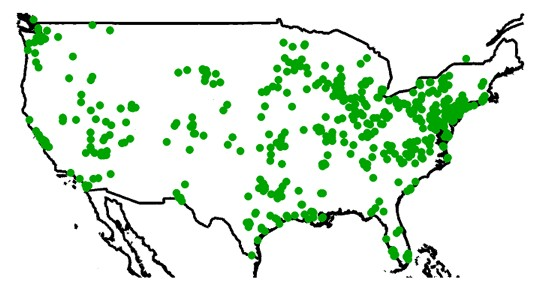
\includegraphics[width = 1\textwidth]{figures/localizationMap.jpg}
\label{fig:localizationMap}
\caption[Map]{Figure \ref{fig:localizationMap} suck!}
\end{figure}

With a dataset this huge, we need

\section{Outline of the Paper}

We have many images from which we need to find interesting variants.  A lot of the variance is controlled, be it through 



